% To convert to svg
% lualatex --output-format=dvi mother.tex
% dvisvgm mother.dvi
% \documentclass[dvisvgm]{minimal}		%uncomment to convert to svg

\documentclass[border=0]{standalone}
\usepackage{tikz}
\usetikzlibrary{intersections,through,calc,shapes.geometric}
\usepackage{xcolor}
\definecolor{highlight2}{HTML}{99cc99}
\begin{document}
    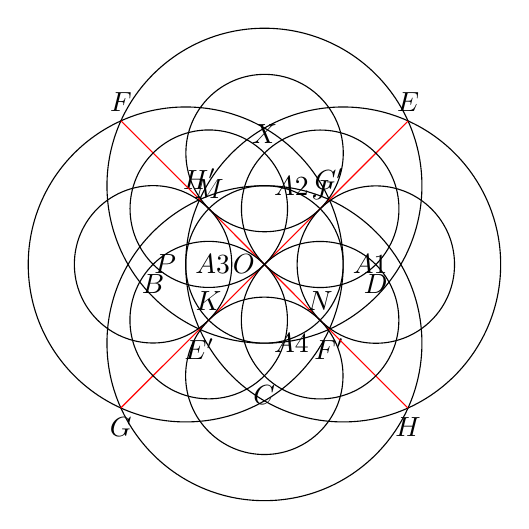
\begin{tikzpicture}
        \pgfmathsetmacro{\r}{1}
        \pgfmathsetmacro{\a}{sqrt(3)}
        \coordinate [label=left:$O$] (O) at (0,0);
        \coordinate [label=right:$A1$] (A1) at (0:\r);
        \coordinate [label=right:$A2$] (A2) at (90:\r);
        \coordinate [label=right:$A3$] (A3) at (180:\r);
        \coordinate [label=right:$A4$] (A4) at (270:\r);
        \node (P) [name path=P,draw,circle through=(A1),label=left:$P$] at (O) {};
        \node (Q) [name path=Q,draw,circle through=(A3)] at (A1) {};
        \node (R) [name path=R,draw,circle through=(A4)] at (A2) {};
        \node (S) [name path=S,draw,circle through=(A1)] at (A3) {};
        \node (T) [name path=T,draw,circle through=(A2)] at (A4) {};
        \path [name intersections={of=Q and R, by={[label=above:$E$]E, [label=below:$E'$]E'}}];
        \path [name intersections={of=R and S, by={[label=above:$F$]F, [label=below:$F'$]F'}}];
        \path [name intersections={of=S and T, by={[label=above:$G'$]G', [label=below:$G$]G}}];
        \path [name intersections={of=T and Q, by={[label=above:$H'$]H', [label=below:$H$]H}}];
        \draw [name path=E--G,red] (E) -- (G);
        \draw [name path=F--H,red] (F) -- (H);
        \path [name intersections={of=E--G and P, by={[label=above:$J$]J,[label=above:$K$]K}}];
        \path [name intersections={of=F--H and P, by={[label=above:$M$]M,[label=above:$N$]N}}];
        \node [name path=Jc,draw,circle through=(O)] at (J) {};
        \node [name path=Kc,draw,circle through=(O)] at (K) {};
        \node [name path=Mc,draw,circle through=(O)] at (M) {};
        \node [name path=Nc,draw,circle through=(O)] at (N) {};
        \path [name intersections={of=Jc and Mc, by={[label=above:$X$]X,X'}}];
        \path [name intersections={of=Kc and Mc, by={B', [label=below:$B$]B}}];
        \path [name intersections={of=Kc and Nc, by={C', [label=below:$C$]C}}];
        \path [name intersections={of=Jc and Nc, by={D', [label=below:$D$]D}}];
        \node [draw,circle through=(J)] at (X) {};
        \node [draw,circle through=(M)] at (B) {};
        \node [draw,circle through=(K)] at (C) {};
        \node [draw,circle through=(N)] at (D) {};
    \end{tikzpicture}
\end{document}
